
%(BEGIN_QUESTION)
% Copyright 2011, Tony R. Kuphaldt, released under the Creative Commons Attribution License (v 1.0)
% This means you may do almost anything with this work of mine, so long as you give me proper credit

This room pressure control system maintains a slightly positive pressure in a precision electronic assembly room to prevent dust from entering from the outside, while always ensuring a rapid flow rate of air through the room.  It regulates pressure by modulating two variable-speed fans: one introducing air to the room (the ``forced draft'' fan) and one venting air from the room (the ``induced draft'' fan).  A pressure transmitter outputs 4 mA at 0 "W.C room pressure and 20 mA at 2 "W.C. room pressure:
 
$$\includegraphics[width=15.5cm]{i00403x01.eps}$$

Suppose you are called to troubleshoot a problem in this system: the room air pressure is holding steady at +1.03 inches WC (according to the display on the DDC control system).  Based on this data, identify the most likely cause of the problem, and also how you would confirm your diagnosis {\it before} making any repairs.

\vskip 20pt \vbox{\hrule \hbox{\strut \vrule{} {\bf Suggestions for Socratic discussion} \vrule} \hrule}

\begin{itemize}
\item{} What does ``VFD'' stand for, and what exactly do the ``VFD'' boxes do to exert control over the speed of the two fan motors?
\item{} Explain why VFD control of air flow into and out of a forced-ventilation building makes more sense than using valve, dampers, or louvers to do the same.
\end{itemize}

\underbar{file i00403}
%(END_QUESTION)





%(BEGIN_ANSWER)

Chances are there is something wrong with the ID fan, causing it to move less air than it should.  Alternatively, the FD fan could be at fault, spinning faster than it should.

%(END_ANSWER)





%(BEGIN_NOTES)

The fact the DCS registers the offset tells us it's not caused by a transmitter problem.  Chances are there is something wrong with the ID fan, causing it to move less air than it should.  Alternatively, the FD fan could be at fault, spinning faster than it should.

\vskip 10pt

A good way to help diagnose this problem is to look at the controller's output to see how hard it is driving the ID fan.

%INDEX% Process: clean room pressure control

%(END_NOTES)


